\documentclass[twocolumn]{article}
\setlength{\columnsep}{.2in}
\usepackage{listings}
\usepackage{color}
\usepackage{amsmath}
\usepackage{algorithm}
\usepackage[noend]{algpseudocode}
\usepackage{graphicx}


\title{Relazione Progetto SCPD}
\date{Dicembre 2022}
\author{Michele Valfrè}
\begin{document}
	\maketitle
	\section{Introduzione: Metodo di Jacobi}
	Il metodo di Jacobi è un metodo iterativo per la soluzione di sistemi di equazioni lineari nella forma $Ax=b$ dove $A$ è una matrice quadrata $n\times n$, $x$ e $b$ sono vettori colonna di dimensione $n$. 
	La condizione generale di convergenza del metodo è che il raggio spettrale, ovvero, nel caso di una matrice quadrata, il massimo valore assoluto dei suoi autovalori, sia minore di $1$.\\
	Tuttavia, condizione sufficiente ma non necessaria per la convergenza del metodo è che $A$ sia diagonalmente dominante, ovvero
	\begin{equation}\label{f1}
		\forall i,\ |a_{ii}| >= \sum_{j \neq i} |a_{ij}| 
	\end{equation}
	
	Il passo $k$-esimo dell' iterazione è descritto dall' equazione
	\begin{equation}\label{f2}
		x^{k}_i = \frac{1}{a_{i,i}}[b_i  - \sum_{j\neq i}a_{i,j}x^{k-1}_j].
	\end{equation}
	\section{Struttura Dati}
	La struttura utilizzata in entrambe le implementazioni è la seguente:
	\lstinputlisting[language=C++,
	emph={int,char,double,float,unsigned,long},
	emphstyle={\color{blue}},
	basicstyle=\ttfamily\scriptsize,
	columns=fullflexible,
	linerange={20-26}]
	{"../src/jacobi.h"} \label{lin_sys_struct}
	Come si può notare, sono mantenuti sia il numero di righe che il numero di colonne di $A$. Si tratta di un' informazione ridondante nel caso dell' implementazione sequenziale(una delle precondizioni è che $A$ sia quadrata), tuttavia, tornerà utile nell' implementazione parallela, dove le singole UC non opereranno su matrici quadrate.
	\section{Algoritmo Sequenziale}
	L' implementazione sequenziale è l' applicazione diretta del metodo: preso un sistema di equazioni lineari $system$, ad ogni iterazione, scorre le righe della matrice $system.A$  ed applica l' equazione \eqref{f2} mantenendo un riferimento al vecchio valore di $system.x$ nella variabile $old\_x$:
	\begin{algorithm}
		\footnotesize
		\caption{Jacobi Sequenziale}
		\begin{algorithmic}[1]
			\Function{JACOBI\_SEQ}{$system$,$iterations$}
				\While{$iterations > 0$}
				\State $old\_x \gets system.x$
				\State $i \gets 0$
				\While{$i < system.rows$}
				\State $sum \gets \sum_{j\neq i} system.A[i] - old\_x[j]$%COMPUTE\_SUM(system,i,old\_x)$
				\State $system.x[i] \gets \frac{1}{system.A[i][i]}(system.b[i] - sum)$
				\State $i \gets i + 1$
				\EndWhile
				\State $iterations \gets iterations - 1$
				\EndWhile
			\EndFunction
		\end{algorithmic}
	\end{algorithm}


	\section{Algoritmo Parallelo}
	Come si può notare dall' equazione \eqref{f2}, i dati necessari per computare la variabile $x_i$ al passo $k$ sono l' $i-$esima riga, il valore $b_i$ corrispondente e l' intero vettore $x$ alla fine del passo $k-1$. Siccome i dati sono immediatamente disponibili,  si è scelto di estrarre il parallelismo dai essi(paradigma data parallel). Si fa notare che la computazione, così trattata, sia di tipo globalmente sincrona: tutte le UC si arrestano alla fine dell' iterazione($Barrier$ implicita data dall' istruzione $MPI_Gatherv$) per consentire il calcolo del nuovo vettore $x$.  Il processo con $rank$ pari a 0 svolge contemporaneamente i ruoli di $Emitter$,  dividendo i dati fra i processi, $Worker$, computando una parte del nuovo valore di $x$, $Collector$, raccogliendo e combinando i risultati alla fine di ogni iterazione. In particolare, l' algoritmo può essere riassunto dai seguenti passi:
	\begin{enumerate}
		\item Il $Master$ divide la matrice $A$ e il vettore $b$ fra i processi secondo la tecnica di bilanciamento del carico $round \ robin$. Così facendo, si delineano due casi:
		\begin{itemize}
			\item se il numero di processi divide esattamente il numero di righe della matrice, il carico è uguale per tutti;
			\item altrimenti, il numero di processi in eccesso(resto della divisione del numero di righe per il numero di processi) sarà comunque distribuito equamente: alcuni processi avranno una riga in più da gestire rispetto agli altri.
		\end{itemize}
	si fa notare come, in quest' ultimo caso, non vi siano particolari miglioramenti in termini di tempo siccome, alla fine di ogni iterazione, è presente una $Barrier$ implicita(vedere passo 4). Ciò comporta che il tempo di esecuzione complessivo sarà limitato dal tempo di esecuzione dei processi più lenti(quelli a cui sono assegnate più righe) e che sia quindi sempre più conveniente scegliere un numero di processi che divida esattamente il numero di righe della matrice $A$.
	\item all' inizio dell' iterazione, il $Master$ distribuisce($MPI\_Bcast$) il vettore $x$ fra tutti i processi;
	\item il processo $n$ applica la formula \eqref{f2} a ognuna delle proprie variabili/righe;
	\item il $Master$ raccoglie i risultati $(MPI\_Gatherv)$ e li combina ottenendo i nuovi valori di $x$ e torna al passo 2.
	\end{enumerate}
	
	La memoria allocata da ogni processo sarà dunque quella destinata a mantenere le proprie porzioni di $A$ e  $b$ e l' intero vettore $x$ computato al passo precedente.
	
	Al fine di evitare l' invio di informazioni ridondanti, invece di distribuire sia l' intero vettore $x$ che la porzione di esso che dovrà essere modificata dal processo, viene comunicato un offset(che sarebbe comunque necessario calcolare per $MPI\_Scatterv$ e $MPI\_Gatherv$) che sarà utilizzato per determinare l' inizio di quest' ultima.
	
	\section{Sperimentazione e Conclusioni}
	La sperimentazione è stata effettuata su una matrice $300\times300$ per 200 iterazioni usando la partizione cineca. Il tempo di esecuzione della versione sequenziale del programma è di $1.999670985\ s$.
	Nel seguente grafico sono mostrati i tempi di esecuzione della versione parallela al variare del numero di processi(da 2 a 32):\\
	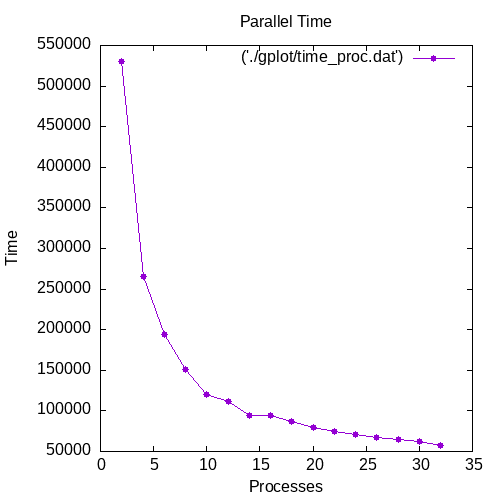
\includegraphics[scale=0.5]{time_proc.png}
	\\
	Come si può notare, il miglioramento più consistente è ottenuto passando da 2 a 4 processi.
	\\Lo speedup, riassunto dal grafico seguente, è essenzialmente lineare:\\
	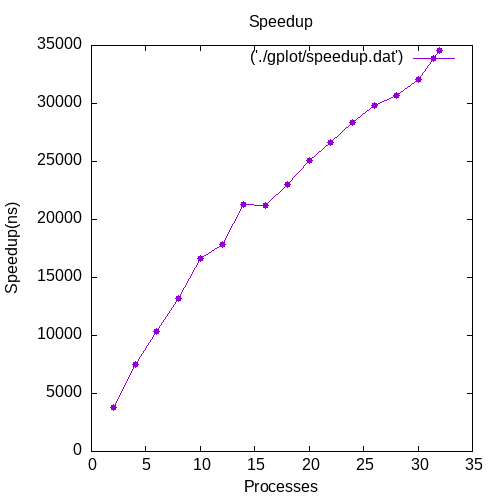
\includegraphics[scale=0.5]{speedup.png}
	\\
	come già discusso in precedenza, i risultati migliori si ottengono quando il numero di processi divide esattamente il numero di righe. La grana computazionale ottima è di una riga per UC.
\end{document}